
%Integrator erweitert

\documentclass{standalone}
\usepackage{circuitikz}
\usepackage{amsmath}

\begin{document}


\begin{circuitikz}[european]
    \ctikzset{bipoles/length=1cm}
    
    \draw
    (0,0) node[op amp] (opamp) {};
    
    \draw (opamp.-) to[R, european resistor, l=$R_1$] (-2, 0.35) -- (-3, 0.35) node[ocirc]{};
    
    \draw [-latex] ([yshift=-2mm] -3,0.35)--(-3,-1.35) node[midway,left] {$U_e$} ; 
   
 % Zeichne C   
    \draw (opamp.-) to[short,*-] ++(0,0.75) coordinate (leftD) to[short,-*](leftD)
    to[C, l=$C$] (leftD -| opamp.out) to[short,-*](leftD -| opamp.out) ;

    \draw [-latex] ([yshift=-2mm] opamp.out)--(0.85,-1.35) node[midway,left] {$U_a$}; 
    
    \draw (0.85,-1.45) node[ocirc]{} to(0.85,-1.5) node[ground]{};
    \draw (-3,-1.45)node[ocirc]{}to(-3,-1.5) node[ground]{};

   \draw (opamp.out)--(2,0) node[ocirc]{};
% Zeichne R2
   \draw (leftD -| opamp.out) to[short,*-](leftD -| opamp.out) to ( opamp.out);

    \draw (opamp.+) -- (-1,-0.35) to (-1,-1.5) node[ground]{};

    
\end{circuitikz}


\end{document}







%Integrator erweitert

\documentclass{standalone}
\usepackage{circuitikz}
\usepackage{amsmath}
\usepackage{siunitx}

\begin{document}

\begin{circuitikz}[european]
    \ctikzset{bipoles/length=1cm}
    
    \draw
    (0,0) node[op amp] (opamp) {};
    
    \draw (opamp.-) to[R, european resistor, l=$R_1$,a=\SI{10}{\kilo\ohm}] (-2, 0.35) -- (-3, 0.35) node[ocirc]{};
    
    \draw [-latex] ([yshift=-2mm] -3,0.35)--(-3,-1.35) node[midway,left] {$U_e$} ; 
   
 % Zeichne C   
    \draw (opamp.-) to[short,*-] ++(0,1.25) coordinate (leftD) to[short,-*](leftD)
    to[C, l=$C$,a=\SI{100}{\nano\farad}] (leftD -| opamp.out) to[short,-*](leftD -| opamp.out) ;

    \draw [-latex] ([yshift=-2mm] opamp.out)--(0.85,-1.35) node[midway,left] {$U_a$}; 
    
    \draw (0.85,-1.45) node[ocirc]{} to(0.85,-1.5) node[ground]{};
    \draw (-3,-1.45)node[ocirc]{}to(-3,-1.5) node[ground]{};

   \draw (opamp.out)--(2,0) node[ocirc]{};
% Zeichne R2
   \draw (opamp.-) to[short,*-] ++(0,2.75) coordinate (leftC)  to[R, l=$R_2$,a=\SI{1}{\mega\ohm}] (leftC -| opamp.out)  to[short,-*] (opamp.out);

    \draw (opamp.+) -- (-1,-0.35) to (-1,-1.5) node[ground]{};

    
\end{circuitikz}

\end{document}



%Tiefpass

%Integrator erweitert

\documentclass{standalone}
\usepackage{circuitikz}
\usepackage{amsmath}
\usepackage{siunitx}

\begin{document}

\begin{circuitikz}[european]
    \ctikzset{bipoles/length=1cm}
    
    \draw
    (0,0) node[op amp] (opamp) {};
    
    \draw (opamp.-) to[R, european resistor, l=$R_1$,a=\SI{10}{\kilo\ohm}] (-2, 0.35) -- (-3, 0.35) node[ocirc]{};
    
    \draw [-latex] ([yshift=-2mm] -3,0.35)--(-3,-1.35) node[midway,left] {$U_e$} ; 
   
 % Zeichne C   
    \draw (opamp.-) to[short,*-] ++(0,1.25) coordinate (leftD) to[short,-*](leftD)
    to[C, l=$C$,a=\SI{100}{\nano\farad}] (leftD -| opamp.out) to[short,-*](leftD -| opamp.out) ;

    \draw [-latex] ([yshift=-2mm] opamp.out)--(0.85,-1.35) node[midway,left] {$U_a$}; 
    
    \draw (0.85,-1.45) node[ocirc]{} to(0.85,-1.5) node[ground]{};
    \draw (-3,-1.45)node[ocirc]{}to(-3,-1.5) node[ground]{};

   \draw (opamp.out)--(2,0) node[ocirc]{};
% Zeichne R2
   \draw (opamp.-) to[short,*-] ++(0,2.75) coordinate (leftC)  to[R, l=$R_2$,a=\SI{10}{\kilo\ohm}] (leftC -| opamp.out)  to[short,-*] (opamp.out);

    \draw (opamp.+) -- (-1,-0.35) to (-1,-1.5) node[ground]{};

    
\end{circuitikz}

\end{document}


% PI Filter

%Integrator erweitert

\documentclass{standalone}
\usepackage{circuitikz}
\usepackage{amsmath}
\usepackage{siunitx}

\begin{document}

\begin{circuitikz}[european]
    \ctikzset{bipoles/length=1cm}
    
    \draw
    (0,0) node[op amp] (opamp) {};
    
    \draw (opamp.-) to[R, european resistor, l=$R_1$,a=\SI{10}{\kilo\ohm}] (-2, 0.35) -- (-3, 0.35) node[ocirc]{};
    
    \draw [-latex] ([yshift=-2mm] -3,0.35)--(-3,-1.35) node[midway,left] {$U_e$} ; 
   
 % Zeichne C   
    \draw (opamp.-) to[short,*-] ++(0,1.25) coordinate (leftD) 
    to[R, l=$R_2$,a=\SI{10}{\kilo\ohm}] (leftD -| opamp.out)  ;

    \draw [-latex] ([yshift=-2mm] 3,0)--(3,-1.35) node[midway,left] {$U_a$}; 
    
    \draw (3,-1.45) node[ocirc]{} to(3,-1.5) node[ground]{};
    \draw (-3,-1.45)node[ocirc]{}to(-3,-1.5) node[ground]{};

   \draw (opamp.out)--(4,0) node[ocirc]{};
% Zeichne R2
   \draw (leftD -| opamp.out)  to[C, l=$C$,a=\SI{100}{\nano\farad}] (3,1.55)  to[short,-*] (3,0);

    \draw (opamp.+) -- (-1,-0.35) to (-1,-1.5) node[ground]{};

    
\end{circuitikz}

\end{document}

%Schmitt-Träger

  \begin{figure}[H]
  \centering
  \begin{circuitikz}[european]

    \ctikzset{bipoles/length=1cm}
    
    \draw
    (0,0) node[op amp,yscale=-1] (opamp) {};
    
    \draw (opamp.+) to[R, european resistor, l=$R_1$] (-2, 0.35) -- (-3, 0.35) node[ocirc]{};
    
    \draw [-latex] ([yshift=-2mm] -3,0.35)--(-3,-1.35) node[midway,left] {$U_e$} ; 
   
  
    \draw (opamp.+) to[short,*-] ++(0,0.75) coordinate (leftD) to[short](leftD)
    to[R, european resistor, l=$R_2$] (leftD -| opamp.out) to [short,-*] (opamp.out) ;

    \draw [-latex] ([yshift=-2mm] opamp.out)--(0.85,-1.35) node[midway,left] {$U_a$}; 
    
    \draw (0.85,-1.45) node[ocirc]{} to(0.85,-1.5) node[ground]{};
    \draw (-3,-1.45)node[ocirc]{}to(-3,-1.5) node[ground]{};

   \draw (opamp.out)--(2,0) node[ocirc]{};
% Zeichne R2

    \draw (opamp.-) -- (-1,-0.35) to (-1,-1.5) node[ground]{};
    %\end{tikzpicture}
\end{circuitikz}
\end{figure}


%Hochpassfilter 
  \begin{figure}[H]
  \centering
\begin{circuitikz}[european]

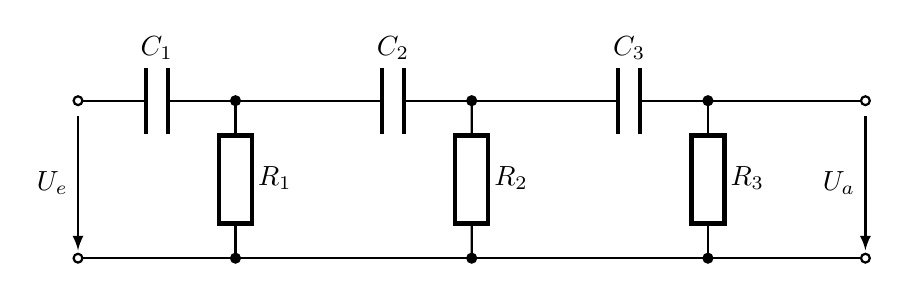
\begin{tikzpicture}[european,thick]
% First Stage
\draw (0,0) node[ocirc]{} to[short] ++(3,0);
\draw (0,2) node[ocirc]{} to[C,l=$C_1$] ++(2,0) coordinate(a);
\draw (a) to[short] ++(1,0);
\draw (a) to[R,l=$R_1$,*-*] ++(0,-2);

% Second Stage
\draw (3,0) to[short] ++(3,0);
\draw (3,2) to[C,l=$C_2$] ++(2,0) coordinate(b);
\draw (b) to[short] ++(1,0);
\draw (b) to[R,l=$R_2$,*-*] ++(0,-2);

% Third Stage
\draw (6,0) to[short] ++(3,0);
\draw (6,2) to[C,l=$C_3$] ++(2,0) coordinate(c)  ;
\draw (8,2) --(10,2) node[ocirc]{};
\draw (c) to[R,l=$R_3$ ,*-*] (8, 0) -- (10, 0) node[ocirc]{};

% Voltage labels

\draw [-latex] ([yshift=-2mm] 0,2)--(0,0.1) node[midway,left] {$U_e$} ;  
\draw [-latex] ([yshift=-2mm] 10,2)--(10,0.1) node[midway,left] {$U_a$};  

\end{tikzpicture}
\end{circuitikz}
\end{figure}

%invertierender Verstärker
\documentclass{article}
\usepackage{circuitikz}
\usepackage{amsmath}
\usepackage{siunitx}

\begin{document}

\begin{circuitikz}[european]
    \ctikzset{bipoles/length=1cm}
    
    \draw
    (0,0) node[op amp] (opamp) {};
    
    \draw (opamp.-) to[R, european resistor, l=$R_5$,a=\SI{10}{\kilo\ohm}] (-2.5, 0.35) -- (-3, 0.35) node[ocirc]{};
    
    \draw [-latex] ([yshift=-2mm] -3,0.35)--(-3,-1.35) node[midway,left] {$U_e$} ; 
   
 % Zeichne C   
    \draw (opamp.-) to[short,*-] ++(0,1.25) coordinate (leftD) 
    to[R, l=$R_4$,a=\SI{10}{\kilo\ohm}] (leftD -| opamp.out)  ;

    \draw [-latex] ([yshift=-2mm] 2,0)--(2,-1.35) node[midway,left] {$U_a$}; 
    
    \draw (2,-1.45) node[ocirc]{} to(2,-1.5) node[ground]{};
    \draw (-3,-1.45)node[ocirc]{}to(-3,-1.5) node[ground]{};

   \draw (opamp.out)--(2,0) node[ocirc]{};
 
   \draw (leftD -| opamp.out) --(1.5,1.55)  to[short,-*] (1.5,0);

    \draw (opamp.+) -- (-1,-0.35) to (-1,-1.5) node[ground]{};

    
\end{circuitikz}

\end{document}

